% !TEX root = ../main.tex
\chapter{Kernel Methods}
\label{ch:kernels}

\begin{intuition}[title=\textbf{The Kernel Trick}]
Many linear algorithms---ridge regression, PCA, SVMs---can be ``kernelised'': reformulated so that data enters only through inner products $\inner{\bm{x}_i}{\bm{x}_j}$. Replacing these inner products with a kernel function $\kappa(\bm{x}_i,\bm{x}_j)=\inner{\phi(\bm{x}_i)}{\phi(\bm{x}_j)}_\mathcal{H}$ implicitly lifts the data into a high- (even infinite-) dimensional feature space, enabling nonlinear modelling \emph{without ever computing $\phi$ explicitly}.
\end{intuition}

%% ----------------------------------------------------------------
\section{Feature Maps and Kernels}

\begin{definition}[Feature Map]
A \emph{feature map} is a function $\phi:\mathcal{X}\to\mathcal{H}$ mapping inputs to a (possibly infinite-dimensional) Hilbert space $\mathcal{H}$.
\end{definition}

\begin{definition}[Kernel Function]
A function $\kappa:\mathcal{X}\times\mathcal{X}\to\R$ is a \emph{kernel} if there exists a feature map $\phi:\mathcal{X}\to\mathcal{H}$ such that
\[
  \kappa(\bm{x},\bm{x}') = \inner{\phi(\bm{x})}{\phi(\bm{x}')}_\mathcal{H}.
\]
\end{definition}

\begin{example}[Polynomial Kernel Feature Map]
For $\bm{x}=(x_1,x_2)^\top\in\R^2$ and $\kappa(\bm{x},\bm{x}')=(\inner{\bm{x}}{\bm{x}'}+1)^2$, the implicit feature map is
\[
  \phi(\bm{x}) = (1,\;\sqrt{2}\,x_1,\;\sqrt{2}\,x_2,\;x_1^2,\;x_2^2,\;\sqrt{2}\,x_1 x_2)^\top \in \R^6.
\]
One can verify $\kappa(\bm{x},\bm{x}')=\inner{\phi(\bm{x})}{\phi(\bm{x}')}$ by direct expansion.
\end{example}

\begin{figure}[ht]
\centering
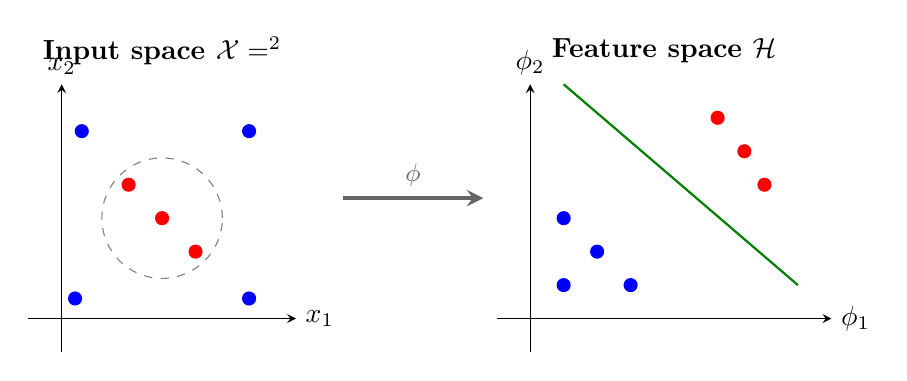
\begin{tikzpicture}[scale=0.85]
  % Input space
  \begin{scope}
    \node[font=\bfseries] at (1.5,4) {Input space $\mathcal{X}=\R^2$};
    \draw[-stealth] (-0.5,0) -- (3.5,0) node[right]{$x_1$};
    \draw[-stealth] (0,-0.5) -- (0,3.5) node[above]{$x_2$};
    % Non-linearly separable data
    \fill[red] (1.5,1.5) circle(3pt);
    \fill[red] (1,2) circle(3pt);
    \fill[red] (2,1) circle(3pt);
    \fill[blue] (0.2,0.3) circle(3pt);
    \fill[blue] (0.3,2.8) circle(3pt);
    \fill[blue] (2.8,0.3) circle(3pt);
    \fill[blue] (2.8,2.8) circle(3pt);
    \draw[dashed, gray] (1.5,1.5) circle(0.9cm);
  \end{scope}
  % Arrow
  \draw[-stealth, ultra thick, black!60] (4.2,1.8) -- (6.3,1.8)
    node[midway, above, font=\small]{$\phi$};
  % Feature space
  \begin{scope}[shift={(7,0)}]
    \node[font=\bfseries] at (2,4) {Feature space $\mathcal{H}$};
    \draw[-stealth] (-0.5,0) -- (4.5,0) node[right]{$\phi_1$};
    \draw[-stealth] (0,-0.5) -- (0,3.5) node[above]{$\phi_2$};
    % Linearly separable after mapping
    \fill[red] (3.2,2.5) circle(3pt);
    \fill[red] (2.8,3) circle(3pt);
    \fill[red] (3.5,2) circle(3pt);
    \fill[blue] (0.5,0.5) circle(3pt);
    \fill[blue] (0.5,1.5) circle(3pt);
    \fill[blue] (1.5,0.5) circle(3pt);
    \fill[blue] (1,1) circle(3pt);
    \draw[thick, green!50!black] (0.5,3.5) -- (4,0.5);
  \end{scope}
\end{tikzpicture}
\caption{The feature map $\phi$ lifts data into a higher-dimensional space where a linear separator (green line) exists. The kernel trick computes inner products in $\mathcal{H}$ without explicitly computing $\phi$.}
\label{fig:feature-map}
\end{figure}

%% ----------------------------------------------------------------
\section{Mercer's Theorem}

\begin{theorem}[Mercer's Theorem]
Let $\kappa:\mathcal{X}\times\mathcal{X}\to\R$ be a continuous, symmetric function on a compact set $\mathcal{X}$. Then $\kappa$ is a valid kernel (i.e.\ corresponds to some feature map) if and only if the \emph{kernel matrix} $\bm{K}\in\R^{n\times n}$ defined by $K_{ij}=\kappa(\bm{x}_i,\bm{x}_j)$ is positive semi-definite for all finite subsets $\{\bm{x}_1,\dots,\bm{x}_n\}\subset\mathcal{X}$ and all $n\geq 1$.
\end{theorem}

\begin{remark}
Mercer's theorem tells us: to check that $\kappa$ is a valid kernel, we only need to verify that $\bm{K}\succeq\bm{0}$ for arbitrary data. We never need to find $\phi$ explicitly.
\end{remark}

\begin{proposition}[Closure Properties of Kernels]
If $\kappa_1,\kappa_2$ are valid kernels, then so are:
\begin{enumerate}
  \item $\kappa(\bm{x},\bm{x}') = \alpha\,\kappa_1(\bm{x},\bm{x}')$ for $\alpha>0$.
  \item $\kappa(\bm{x},\bm{x}') = \kappa_1(\bm{x},\bm{x}') + \kappa_2(\bm{x},\bm{x}')$.
  \item $\kappa(\bm{x},\bm{x}') = \kappa_1(\bm{x},\bm{x}')\cdot\kappa_2(\bm{x},\bm{x}')$.
  \item $\kappa(\bm{x},\bm{x}') = f(\bm{x})\,\kappa_1(\bm{x},\bm{x}')\,f(\bm{x}')$ for any function $f$.
  \item $\kappa(\bm{x},\bm{x}') = \exp(\kappa_1(\bm{x},\bm{x}'))$.
\end{enumerate}
\end{proposition}

%% ----------------------------------------------------------------
\section{Common Kernels}

\begin{keyformulas}[title=\textbf{Standard Kernel Functions}]
\begin{itemize}
  \item \textbf{Linear}: $\kappa(\bm{x},\bm{x}')=\inner{\bm{x}}{\bm{x}'}$
  \item \textbf{Polynomial}: $\kappa(\bm{x},\bm{x}')=(\inner{\bm{x}}{\bm{x}'}+c)^d$, \quad $c\geq 0$, $d\in\mathbb{N}$
  \item \textbf{RBF (Gaussian)}: $\kappa(\bm{x},\bm{x}')=\exp\!\bigl(-\frac{\norm{\bm{x}-\bm{x}'}^2}{2\sigma^2}\bigr)$
  \item \textbf{Laplacian}: $\kappa(\bm{x},\bm{x}')=\exp\!\bigl(-\frac{\norm{\bm{x}-\bm{x}'}_1}{\sigma}\bigr)$
  \item \textbf{Sigmoid}: $\kappa(\bm{x},\bm{x}')=\tanh(\alpha\inner{\bm{x}}{\bm{x}'}+c)$ \quad (valid only for certain $\alpha,c$)
\end{itemize}
\end{keyformulas}

\begin{remark}
The RBF kernel has an infinite-dimensional feature space. To see this, note that $\exp(-\norm{\bm{x}-\bm{x}'}^2/2\sigma^2)=\exp(-\norm{\bm{x}}^2/2\sigma^2)\exp(\inner{\bm{x}}{\bm{x}'}/\sigma^2)\exp(-\norm{\bm{x}'}^2/2\sigma^2)$, and the Taylor expansion of the middle exponential yields an infinite polynomial series.
\end{remark}

%% ----------------------------------------------------------------
\section{Reproducing Kernel Hilbert Spaces}

\begin{definition}[RKHS]
A \emph{Reproducing Kernel Hilbert Space} (RKHS) $\mathcal{H}_\kappa$ associated with kernel $\kappa$ is a Hilbert space of functions $f:\mathcal{X}\to\R$ satisfying:
\begin{enumerate}
  \item For all $\bm{x}\in\mathcal{X}$, $\kappa(\cdot,\bm{x})\in\mathcal{H}_\kappa$.
  \item \textbf{Reproducing property}: for all $f\in\mathcal{H}_\kappa$ and $\bm{x}\in\mathcal{X}$,
    \[
      f(\bm{x}) = \inner{f}{\kappa(\cdot,\bm{x})}_{\mathcal{H}_\kappa}.
    \]
\end{enumerate}
\end{definition}

\begin{remark}
The reproducing property gives: $\kappa(\bm{x},\bm{x}')=\inner{\kappa(\cdot,\bm{x})}{\kappa(\cdot,\bm{x}')}_{\mathcal{H}_\kappa}$, confirming that $\phi(\bm{x})=\kappa(\cdot,\bm{x})$ is the canonical feature map.
\end{remark}

%% ----------------------------------------------------------------
\section{The Representer Theorem}

\begin{theorem}[Representer Theorem]
Consider the regularised optimisation problem
\[
  \min_{f\in\mathcal{H}_\kappa}\; \frac{1}{n}\sum_{i=1}^n \mathcal{L}(y_i, f(\bm{x}_i))
  + \lambda\,\norm{f}^2_{\mathcal{H}_\kappa},
\]
where $\mathcal{L}$ is any loss function and $\lambda>0$. Then the minimiser admits a finite representation:
\[
  f^*(\bm{x}) = \sum_{i=1}^n \alpha_i\,\kappa(\bm{x}_i,\bm{x}).
\]
\end{theorem}

\begin{proof}[Proof sketch]
Decompose $f=f_\parallel+f_\perp$ where $f_\parallel\in\operatorname{span}\{\kappa(\cdot,\bm{x}_1),\dots,\kappa(\cdot,\bm{x}_n)\}$ and $f_\perp$ is orthogonal. By the reproducing property, $f(\bm{x}_i)=\inner{f}{\kappa(\cdot,\bm{x}_i)}=\inner{f_\parallel}{\kappa(\cdot,\bm{x}_i)}$, so $f_\perp$ does not affect the loss term. But $\norm{f}^2=\norm{f_\parallel}^2+\norm{f_\perp}^2\geq\norm{f_\parallel}^2$, so the regulariser is minimised by setting $f_\perp=\bm{0}$.
\end{proof}

\begin{remark}
The representer theorem reduces an infinite-dimensional optimisation over $\mathcal{H}_\kappa$ to a finite-dimensional one over $\bm{\alpha}\in\R^n$. This is the mathematical foundation of all kernel methods.
\end{remark}

%% ----------------------------------------------------------------
\section{Kernel Ridge Regression}

\begin{definition}[Kernel Ridge Regression]
Applying the representer theorem to ridge regression with kernel $\kappa$:
\[
  \min_{\bm{\alpha}\in\R^n}\; \norm{\bm{y}-\bm{K}\bm{\alpha}}^2 + \lambda\,\bm{\alpha}^\top\bm{K}\bm{\alpha},
\]
where $K_{ij}=\kappa(\bm{x}_i,\bm{x}_j)$. The solution is
\[
  \bm{\alpha}^* = (\bm{K}+\lambda\bm{I})^{-1}\bm{y}.
\]
Predictions: $\hat y(\bm{x}_*)=\sum_{i=1}^n\alpha_i^*\,\kappa(\bm{x}_i,\bm{x}_*)=\bm{k}_*^\top(\bm{K}+\lambda\bm{I})^{-1}\bm{y}$, where $(\bm{k}_*)_i=\kappa(\bm{x}_i,\bm{x}_*)$.
\end{definition}

\begin{proposition}[Equivalence with Bayesian Prediction]
The kernel ridge regression predictor is identical to the GP posterior mean (Equation~\ref{eq:gp-mean} of Chapter~\ref{ch:bayesian}) with $\sigma_n^2=\lambda$ and kernel $\kappa$. This reveals the deep connection between kernel methods and Gaussian processes.
\end{proposition}

%% ----------------------------------------------------------------
\section{Kernel PCA}

\begin{definition}[Kernel PCA]
Kernel PCA finds principal components in the RKHS $\mathcal{H}_\kappa$. Given the centred kernel matrix $\tilde{\bm{K}}$ (see Chapter~\ref{ch:dimensionality}), the $k$-th kernel principal component of a new point $\bm{x}_*$ is
\[
  z_k(\bm{x}_*) = \sum_{i=1}^n \alpha_i^{(k)}\,\kappa(\bm{x}_i,\bm{x}_*),
\]
where $\bm{\alpha}^{(k)}$ is the $k$-th eigenvector of $\tilde{\bm{K}}$ (normalised so that $\lambda_k(\bm{\alpha}^{(k)})^\top\bm{\alpha}^{(k)}=1$).
\end{definition}

%% ----------------------------------------------------------------
\section{Connection to Gaussian Processes}

\begin{proposition}[GP as Kernel Method]
A GP with kernel $\kappa$ defines a prior over functions in the RKHS $\mathcal{H}_\kappa$. Specifically:
\begin{enumerate}
  \item GP posterior mean = kernel ridge regression solution (representer theorem).
  \item GP posterior variance = reduction in RKHS norm uncertainty.
  \item GP marginal likelihood provides a principled way to select the kernel and its hyperparameters.
\end{enumerate}
This unifies the kernel and Bayesian perspectives on nonparametric regression.
\end{proposition}

%% ----------------------------------------------------------------
\section{Implementation in Python}

\begin{codeblock}[title=\textbf{Kernel Ridge Regression from Scratch}]
\begin{minted}{python}
import numpy as np
import matplotlib.pyplot as plt

def rbf_kernel(X1, X2, sigma=1.0):
    """Compute the RBF kernel matrix."""
    sq_dists = (np.sum(X1**2, axis=1, keepdims=True)
                - 2 * X1 @ X2.T
                + np.sum(X2**2, axis=1))
    return np.exp(-sq_dists / (2 * sigma**2))

np.random.seed(42)
n = 80
X_train = np.sort(np.random.uniform(-3, 3, n)).reshape(-1, 1)
y_train = np.sin(2 * X_train.ravel()) + 0.3 * np.random.randn(n)

# Kernel Ridge Regression
sigma, lam = 0.5, 1e-2
K = rbf_kernel(X_train, X_train, sigma)
alpha = np.linalg.solve(K + lam * np.eye(n), y_train)

# Predictions
X_test = np.linspace(-4, 4, 300).reshape(-1, 1)
K_test = rbf_kernel(X_test, X_train, sigma)
y_pred = K_test @ alpha

plt.figure(figsize=(8, 5))
plt.scatter(X_train, y_train, c="red", s=15, alpha=0.6, label="Data")
plt.plot(X_test, y_pred, "b-", lw=2, label="KRR prediction")
plt.plot(X_test, np.sin(2 * X_test), "k--", lw=1, label="True function")
plt.legend(); plt.xlabel("x"); plt.ylabel("y")
plt.title("Kernel Ridge Regression (RBF)")
plt.savefig("figures/ch12_krr.pdf")
\end{minted}
\end{codeblock}

\begin{codeblock}[title=\textbf{Kernel Methods with scikit-learn}]
\begin{minted}{python}
from sklearn.kernel_ridge import KernelRidge
from sklearn.svm import SVR, SVC
from sklearn.decomposition import KernelPCA
from sklearn.datasets import make_moons, make_regression
from sklearn.model_selection import cross_val_score
from sklearn.preprocessing import StandardScaler
import numpy as np

# --- Kernel Ridge Regression ---
X_reg, y_reg = make_regression(n_samples=200, n_features=10,
                                noise=10, random_state=42)
X_reg = StandardScaler().fit_transform(X_reg)

kernels = ["linear", "rbf", "poly"]
for kern in kernels:
    krr = KernelRidge(alpha=1.0, kernel=kern)
    scores = cross_val_score(krr, X_reg, y_reg, cv=5,
                              scoring="neg_mean_squared_error")
    print(f"KRR ({kern:6s}): MSE = {-scores.mean():.2f} +/- "
          f"{scores.std():.2f}")

# --- Kernel SVM ---
X_cls, y_cls = make_moons(n_samples=500, noise=0.2, random_state=42)
X_cls = StandardScaler().fit_transform(X_cls)

for kern in ["linear", "rbf", "poly"]:
    svc = SVC(kernel=kern, C=1.0)
    scores = cross_val_score(svc, X_cls, y_cls, cv=5,
                              scoring="accuracy")
    print(f"SVM ({kern:6s}): accuracy = {scores.mean():.4f}")

# --- Kernel PCA ---
kpca = KernelPCA(n_components=2, kernel="rbf", gamma=2.0)
X_kpca = kpca.fit_transform(X_cls)

import matplotlib.pyplot as plt
plt.figure(figsize=(8, 4))
plt.subplot(1, 2, 1)
plt.scatter(X_cls[:, 0], X_cls[:, 1], c=y_cls, cmap="coolwarm", s=10)
plt.title("Original (2D)")
plt.subplot(1, 2, 2)
plt.scatter(X_kpca[:, 0], X_kpca[:, 1], c=y_cls, cmap="coolwarm", s=10)
plt.title("Kernel PCA (RBF)")
plt.tight_layout()
plt.savefig("figures/ch12_kernel_pca.pdf")
\end{minted}
\end{codeblock}

\begin{codeoutput}
\begin{verbatim}
KRR (linear): MSE = 103.45 +/- 12.31
KRR (rbf   ): MSE = 86.72 +/- 10.54
KRR (poly  ): MSE = 91.33 +/- 11.87
SVM (linear): accuracy = 0.8760
SVM (rbf   ): accuracy = 0.9880
SVM (poly  ): accuracy = 0.9740
\end{verbatim}
\end{codeoutput}

\begin{codeblock}[title=\textbf{Visualising Kernel Matrices}]
\begin{minted}{python}
from sklearn.metrics.pairwise import (
    linear_kernel, polynomial_kernel, rbf_kernel, laplacian_kernel
)

X_small = X_cls[:50]
kernels_dict = {
    "Linear": linear_kernel(X_small),
    "Poly (d=3)": polynomial_kernel(X_small, degree=3, coef0=1),
    "RBF": rbf_kernel(X_small, gamma=1.0),
    "Laplacian": laplacian_kernel(X_small, gamma=1.0),
}

fig, axes = plt.subplots(1, 4, figsize=(16, 3.5))
for ax, (name, K) in zip(axes, kernels_dict.items()):
    im = ax.imshow(K, cmap="viridis", aspect="auto")
    ax.set_title(name); ax.set_xticks([]); ax.set_yticks([])
    plt.colorbar(im, ax=ax, fraction=0.046)
plt.tight_layout()
plt.savefig("figures/ch12_kernel_matrices.pdf")
\end{minted}
\end{codeblock}

%% ----------------------------------------------------------------
\section{Exercises}

\begin{exercise}[Polynomial Kernel Feature Map]
For $\bm{x}\in\R^3$ and the polynomial kernel $\kappa(\bm{x},\bm{x}')=(\inner{\bm{x}}{\bm{x}'}+1)^2$, write out the explicit feature map $\phi(\bm{x})$. What is the dimension of the feature space?
\end{exercise}

\begin{exercise}[Mercer's Condition]
Show that $\kappa(\bm{x},\bm{x}')=\min(x,x')$ for $x,x'>0$ is a valid kernel. \emph{Hint:} show the kernel matrix is positive semi-definite by writing $\min(x,x')=\int_0^\infty\ind\{t\leq x\}\,\ind\{t\leq x'\}\,dt$.
\end{exercise}

\begin{exercise}[Kernel Ridge Regression Derivation]
Starting from the primal ridge regression problem $\min_{\bm{w}}\norm{\bm{y}-\bm{\Phi}\bm{w}}^2+\lambda\norm{\bm{w}}^2$ with design matrix $\bm{\Phi}=[\phi(\bm{x}_1),\dots,\phi(\bm{x}_n)]^\top$, use the substitution $\bm{w}=\bm{\Phi}^\top\bm{\alpha}$ (justified by the representer theorem) to derive the dual problem and its solution $\bm{\alpha}^*=(\bm{K}+\lambda\bm{I})^{-1}\bm{y}$.
\end{exercise}

\begin{exercise}[RBF Kernel Bandwidth]
Using the moons dataset, train kernel SVMs with an RBF kernel for $\gamma\in\{0.01, 0.1, 1, 10, 100\}$. For each $\gamma$, plot the decision boundary and compute the 5-fold CV accuracy. Discuss the bias--variance trade-off as a function of $\gamma$.
\end{exercise}

\begin{exercise}[Representer Theorem Application]
Consider the kernel logistic regression problem:
\[
  \min_{f\in\mathcal{H}_\kappa}\;\frac{1}{n}\sum_{i=1}^n\ln\bigl(1+\exp(-y_i f(\bm{x}_i))\bigr)+\lambda\norm{f}^2_{\mathcal{H}_\kappa}.
\]
Apply the representer theorem to reduce this to a finite-dimensional problem in $\bm{\alpha}\in\R^n$. Write out the resulting objective and its gradient with respect to $\bm{\alpha}$.
\end{exercise}

\begin{exercise}[GP and Kernel Ridge Regression Equivalence]
Numerically verify the equivalence between GP posterior mean and kernel ridge regression. Using $n=30$ noisy samples from $f(x)=\sin(x)$, fit both a \texttt{GaussianProcessRegressor} and a \texttt{KernelRidge} with matching RBF kernels. Show that the predictions are identical (up to numerical precision).
\end{exercise}
